% Chapter 4

\chapter{The rugged virion} % Main chapter title

\label{Chapter4} % For referencing the chapter elsewhere, use \ref{Chapter2} 


%----------------------------------------------------------------------------------------


\section{Physicochemical Properties}
\label{Physicoprop}
The extracellular infectious virus entity is defined as virion. An infectious parvovirus virion only consists of two components, namely of about 75~\% protein and 25~\% DNA. Their molecular weight (MW) is approximately 5.5-6.2~$\times$~10\textsuperscript{6} dalton. The virion buoyant density is 1.39 to 1.43 gcm\textsuperscript{-3}, measured in CsCl gradients \cite{CsCl, pmid4317344}. Since parvoviruses are devoid of a lipid envelope, mature virions are stable in the presence of lipid solvents. In particular, animal parvoviruses show considerable heat resistance. Most species resist alcohol or ether treatment, exposure to pH 3-10, or incubation at 60 \textcelsius~ for 60 min \cite{pmid12935806, pmid12385412, pmid17880601, pmid19039515, pmid14660623, pmid10941577, pmid10662625}, hence they are clearly more stable compared to most other, especially enveloped, viruses. Only harsh conditions, such as treatment with formalin, $\beta$-propiolacetone, hydroxylamine, ultraviolet light, and oxidizing agents as for example sodium hypochlorite, ensure effective virus inactivation \cite{pmid4213983, pmid3416941, pmid7848502, pmid1520981}. Accordingly, the capsid effectively protects the fragile, condensed genome from detrimental biological, chemical, and physical agents, thus ensuring efficient transmission of the virion through the extracellular environment.     

\section{Atomic Model}
\label{Structure}
Currently, there is no crystal structure available for MVMp DNA containing particles. Only baculovirus-expressed MVMp-like particles and empty capsids (ECs) have been determined at a resolution of 3.25 \r{A} and 3.75 \r{A}, respectively \cite{pmid16103145}. For MVMi both DNA-containing full and empty particles were crystallized and determined at 3.5 \r{A} resolution. The known CPV structure \cite{pmid3379641} was used as a phasing model with 52~\% of the 587 amino acids in VP2 of MVMi being identical to CPV. Following molecular replacement and refinement, the resulting electron density map was interpreted with respect to the amino acid sequence of MVMi. The polypeptide chain of the major structural protein, VP2, could be traced from residue 39 to residue 587 at the C-terminus (see Figure~\ref{Structure1}, p.~\pageref{Structure1}) \cite{pmid15299974}. The N-terminal extensions of VP1 and VP2 are not visible in the electron density map. The capsid displays a T=1 icosahedral symmetry, thus having a 5-3-2 point group symmetry containing 31 rotational symmetry axes that intersect at the center: six fivefolds, ten threefolds, and fifteen twofolds. The C-terminal part in common of the structural proteins has an eight-stranded ($\beta$B to $\beta$I) antiparallel $\beta$-barrel topology, referred to as jellyroll motif (reviewed in \cite{pmid2673017, Fundamental_Virology}). This structural motif is frequently found in other virus capsid proteins. Additionally, like many other viruses, parvoviruses have a ninth $\beta$A-strand which is hydrogen-bonded to the $\beta$B-strand. The high structural conservation of the jellyroll motif among parvoviruses is remarkable considering the low sequence homology between members of this family. Large loops between the $\beta$-strands of the $\beta$-barrel that form the principal surface features, particularly the threefold spikes, confer the surface biological properties of the capsid, such as determination of host tropism \cite{pmid1316457, pmid3942033} and sites of antigenicity \cite{pmid8985402, pmid1942246}. Such loops were found to be quite dissimilar in different parvoviruses (see Figure~\ref{Structure1}, p.~\pageref{Structure1}) \cite{pmid8503170}. 

The lack of the first 38 amino acids of VP2 indicates a highly disordered structure for N-VP2 \cite{pmid15299974}. Indeed, a glycine-rich conserved sequence at the N-terminal part of VP2 contributes to its flexibility. In virions, but not in ECs, additional density seen within the fivefold channels was modeled and found to represent the predominantly poly-glycine conserved sequence \cite{pmid15299494, pmid8969301}. These findings suggest that the N-terminus of VP2 is highly dynamic as DNA packaging triggers externalization of one in five N-termini along the pores of the fivefold axis \cite{pmid9817841}.
 
A substantial amount of electron density in the capsid interior was built as 10 DNA nucleotides which were located at equivalent positions to those previously found in the analysis of the structure of CPV \cite{pmid7735832, pmid1616694}. For MVM, 19 additional nucleotides were identified in a difference electron-density map with respect to the data of empty particles. Altogether, these 29 ordered, or partially ordered, nucleotides per icosahedral asymmetric unit imply that approximately 34~\% of the total viral genome display icosahedral symmetry. These findings, and the conservation between the base-binding sites of MVMi and CPV, has led to the identification of a DNA-recognition site on the parvoviral capsid interior \cite{pmid9817841}.    

\begin{figure}
\centering
  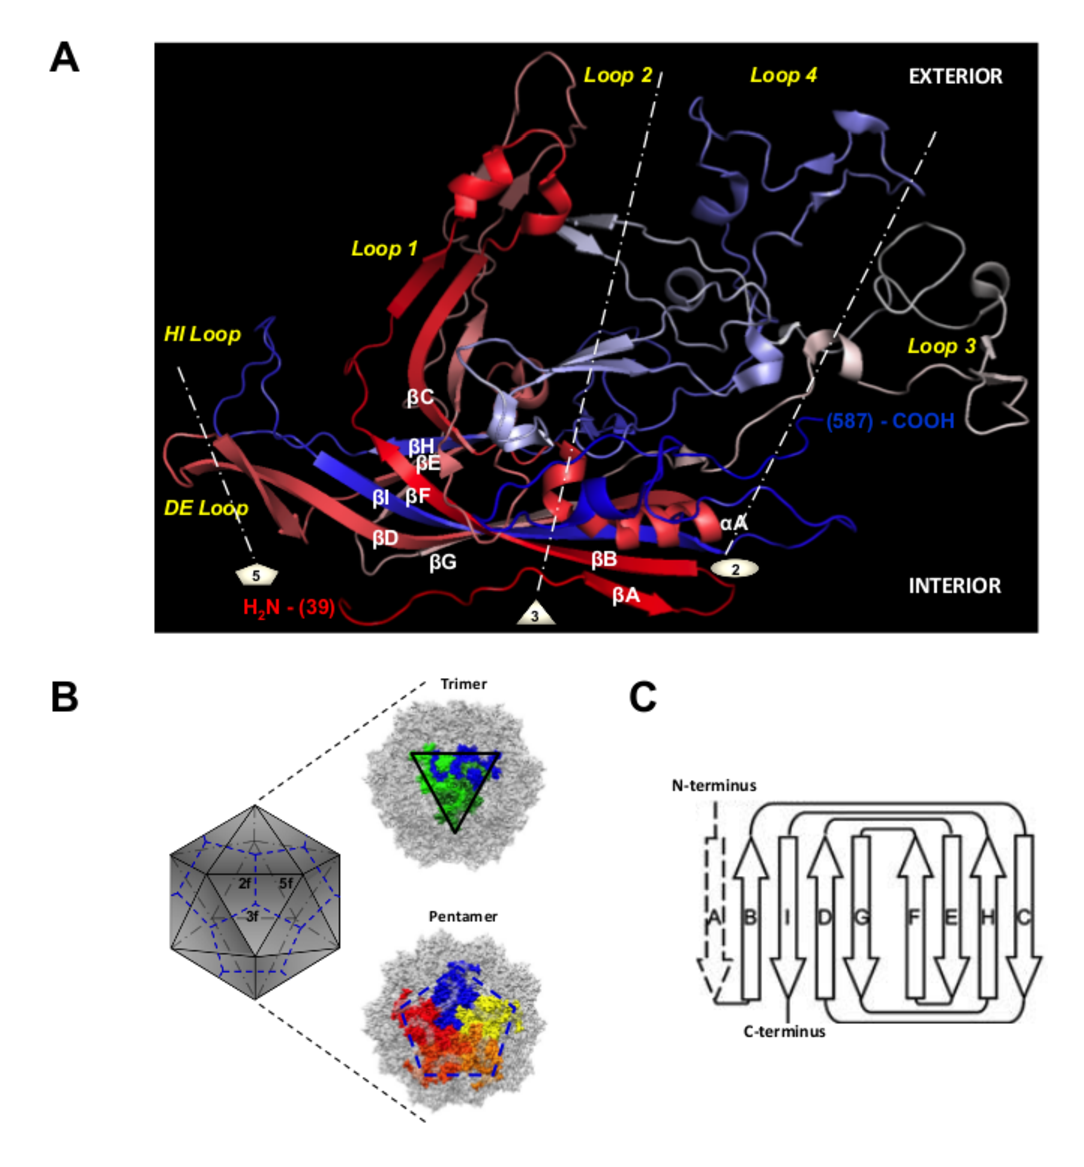
\includegraphics[scale=0.55]{Structure}
  \caption[Structure of MVM]
   {Atomic model of MVM. \textbf{(A)} Ribbon diagram of MVMp VP2 illustrating $\beta$-strands, helical and loop regions. The amino acid sequence is gradually colored in a red–white–blue spectrum, beginning at residue 39 and ending at the C-terminal residue 587. The highly conserved $\alpha$A-helix $\beta$-barrel motif, consisting of two antiparallel $\beta$-sheets ($\beta$ABIDG–$\beta$FEHC), are labeled. The icosahedral twofold (oval), threefold (triangle), and fivefold (pentagon) axes are indicated. Atomic coordinates for MVMp were obtained from RSCB protein database (PDB accession number 1Z14). The illustration was generated using the PyMol program \cite{PyMol}. \textbf{(B)} 60 copies of the capsid proteins form a T=1 icosahedral structure. Each triangle of the icosadeltahedron designates a virus capsid protein subunit. Rotational symmetry axes are referred to as 5f, 3f and 2f, representing 5-folds, 3-folds, and 2-folds, respectively. A VP trimer (assembly intermediate) and a VP pentamer are represented on the right hand side, superimposed on the capsid surface. The representation was generated using the UCSF-Chimera program \cite{pmid15264254} by computing the same atomic coordinates as mentioned in (A). \textbf{(C)} The connectivity of the antiparallel $\beta$ strands (arrows) of the jellyroll $\beta$-barrel is schematically indicated. Strand A is dashed because it is conserved among parvoviruses and a number of other viruses but it is not present in all viruses. This illustration was adapted from \cite{Structure}} 
\label{Structure1}
\end{figure}

%\textit{In vitro}, trypsin digestion of full MVM virions results in a truncated VP3 polypeptide that still contains the glycine-rich sequence. In this way, most VP2 N-termini can be cleaved. These findings suggest that there is a dynamic situation at the fivefold channel. In one model, one in five amino termini are externalized along the fivefold axes and are accessible for cleavage. Newly created, cleaved N-VP3 termini could withdraw into the virion and be replaced at the surface by an uncleaved N-VP2 terminus. \cite{pmid8503170, pmid9817841}.

\section{Structural Proteins}
\label{VPs}

The MVM capsid is made up of 60 copies of a single polypeptide sequence. The virion contains structural proteins of three size classes (VP1-VP3) that constitute a nested set. These share the same C-terminal core structure, but differ in the sequence length on their N-termini. The capsid is assembled from about 10 copies per particle of VP1 (83 kDa), whereas VP2 (64 kDa) represents the major species \cite{pmid988192}. In DNA containing virions, the N-terminal region of VP2 is cleaved during cell entry by intracellular proteolytic digestion to generate VP3 (60 kDa), which displays a truncation of approximately 25 amino acids at its N-terminus (see Section~\ref{Rearrangements}, p.~\pageref{Rearrangements}) \cite{pmid864702, pmid1448928, pmid982825, pmid9770425}. The N-terminal cleavage of VP2 does not occur in ECs, suggesting that DNA packaging into the particle allows the N-VP2 terminus to be externalized \cite{pmid3296697, pmid6481856, pmid864702}. The processing of VP2 in full virions can be mimicked \textit{in vitro} by digestion with tryptic proteases, as for instance chymotrypsin or trypsin. However, the proteolytic site \textit{in vivo} is different to the chymotrypsin- or trypsin-sensitive site \cite{pmid6481856, pmid864702, pmid1448928}. Although containing the identical amino acid sequence that is cleaved in VP2, VP1 does not appear to be cleaved at this position in either type of particle, \textit{in vivo} or \textit{in vitro}. VP2 is both necessary and sufficient for the assembly and encapsidation of viral ssDNA (see Sections~\ref{Assembly} and~\ref{Packaging}, p.~\pageref{Assembly}~-~\pageref{Packaging}) \cite{pmid10662625}. However, VP1 is required to produce an infectious particle since capsids that lack VP1 were blocked subsequent to cell binding and prior to the initiation of DNA replication, thus they are unable to fulfill a complete viral life cycle \cite{pmid8416366}. Indeed, the 142 amino acid N-terminal extension of VP1 which is referred to as VP1 unique region (VP1u) harbors several important motifs to initiate viral infection. Two of which are a PLA\textsubscript{2} motif as well as a nuclear localization signal (NLS), elaborated in Section~\ref{Motif}, p.~\pageref{Motif}. Since VP1u initially is sequestered within the viral shell, the incoming virion must undergo important structural changes \textit{in vivo} in order to expose its functional domains on the capsid surface. By treatment of purified virions under controlled temperature or with urea, VP1u exposure could be demonstrated \textit{in vitro} \cite{pmid9927584, pmid15194745}. 
    
\section{Functional Domains}
\label{Motif}

From the atomic model of parvoviruses it can be estimated that structural proteins of 25-30 kDa theoretically suffice to constitute a capsid to protect the viral genome. However, this minimum size is generally enlarged among parvoviruses. VP1 and VP2 exceed the minimum size more than twice as much. The additional parts of the structural proteins harbor essential functional motifs that mediate a number of processes in the infectious viral life cycle. These include host cell surface receptor recognition (see Section~\ref{Binding}, p.~\pageref{Binding}), entry and escape from endosomes (see Sections~\ref{Endocytosis} to~\ref{Escape}, pp.~\pageref{Endocytosis} -~\pageref{Escape}), nuclear localization (see Section~\ref{Localization}, p.~\pageref{Localization}), DNA packaging, nuclear export, tropism and pathogenicity determinants (see Chapter~\ref{Chapter5}, p.~\pageref{Chapter5}), immune surveillance and final maturation of particles to produce infectious virus progeny \cite{PLA2}.    

\subsection{The Phospholipase A\textsubscript{2} (PLA\textsubscript{2}) Motif}
\label{PLA2}

In the VP1u region of all parvoviruses, except AMDV and the members of the genus \textit{Brevidensovirus}, as well as \textit{Tetraparvovirus}, a PLA\textsubscript{2} motif has been identified \cite{pmid11702787}. The calcium binding loop (YXGXG) and the catalytic histidine-aspartic acid dyad (HDXXY) of parvoviral phospholipases are related to Ca\textsuperscript{2+}-dependent extracellular or secretory sPLA\textsubscript{2}s which are found for example in bee and snake venoms. Unlike all previously characterized sPLA\textsubscript{2}s, the viral sPLA\textsubscript{2} motifs show very weak sequence similarity and lack the characteristic multiple disulfide bonds, thus analogy is mainly restricted to the catalytic units. PLA\textsubscript{2}s specifically catalyze the hydrolysis of phospholipid substrates at the 2-acyl ester (\textit{sn}-2) position to release free fatty acids and lysophospholipids. The viral sPLA\textsubscript{2}s hydrolyze all major classes of glycerophospholipids, except phosphatidylinositol, without displaying a preference for unsaturated \textit{versus} saturated \textit{sn}-2 fatty acyl chains \cite{pmid14726513}. The catalytic activity of the PLA\textsubscript{2} is dependent on Ca\textsuperscript{2+} in mM concentrations and reaches a maximum at a pH range 6-7, presumably associated with the deprotonation of the His residue in the catalytic dyad at such pH \cite{pmid9115999, pmid7574497}.

The biological importance of the viral PLA\textsubscript{2} motif was demonstrated by mutational analyses with AAV2, MVM, and PPV \cite{pmid16284249, pmid11702787, pmid20974479}. Viruses lacking a functional PLA\textsubscript{2} motif were not infectious as they failed to escape from endosomes \cite{pmid16284249, pmid14644609,  pmid11799199, pmid11961250}.               

\begin{figure}
\centering
  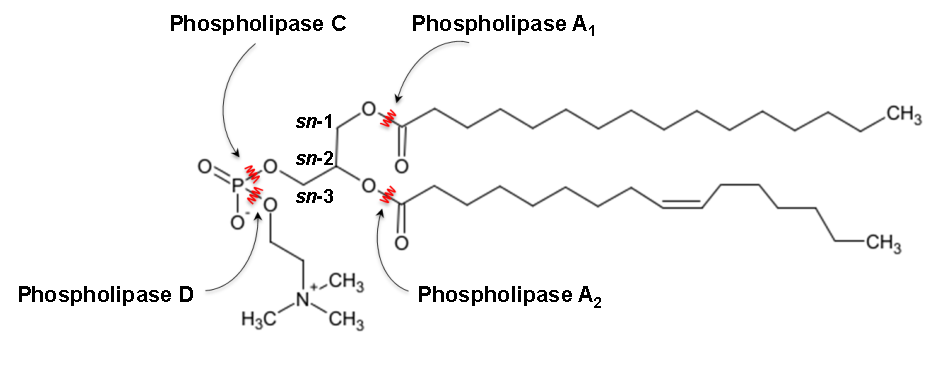
\includegraphics[scale=0.7]{PLA}
  \caption[The cleavage sites of different types of PLAs]
   {The cleavage sites of the different PLAs are illustrated using phosphatidylcholine (PC), a common phospholipid, as an example. Phospholipase A\textsubscript{1}, A\textsubscript{2}, C, and D specifically cleave different ester bonds in the phospholipid. Their respective sites of attack are represented by red staggered lines.} 
\label{PLA}
\end{figure}

\subsection{The Nuclear Localization Signal (NLS)}
\label{NLS1}
In addition to the PLA\textsubscript{2} motif \cite{pmid11702787}, the VP1u region of MVM contains four basic clusters (BCs) of amino acids, referred to as BC1 to BC4. These are highly conserved among parvoviruses and moreover, even in some other DNA viruses. BC1 and BC2 represent conventional NLS which are characterized by a short stretch of basic amino acids \cite{pmid6096007, pmid6088992}. BC3 and BC4, which are separated by a short spacing sequence in between, may rather be arranged as a bipartite NLS domain \cite{pmid1991323}. The clustered basic amino acids interact with transport receptors of the importin/karyopherin family which mediate nuclear import \cite{pmid9126736, pmid9759490, pmid12067655}. Nuclear transport activity has been demonstrated for BC1 in the context of a singly expressed VP1 protein \cite{pmid12072505} and as NLS-peptide coupled to an heterologous carrier protein \cite{pmid9428689}. Furthermore, it is proven to be essential for CPV infectivity \cite{pmid11799183} and for MVM to initiate infection \cite{pmid12072505}. In contrast, BC3 and BC4 did not show such capacity to import VP1 either expressed alone \cite{pmid9428689} or in the context of the complete MVM genome \cite{pmid12072505}. Alternatively, these BCs may be involved in the tethering of the ssDNA genome to the capsid inner surface. Such function has been demonstrated for two basic, significantly homologous DNA-binding domains of the protein J of the $\phi$X174 bacteriophage \cite{pmid11991963}.

\begin{figure}
\centering
  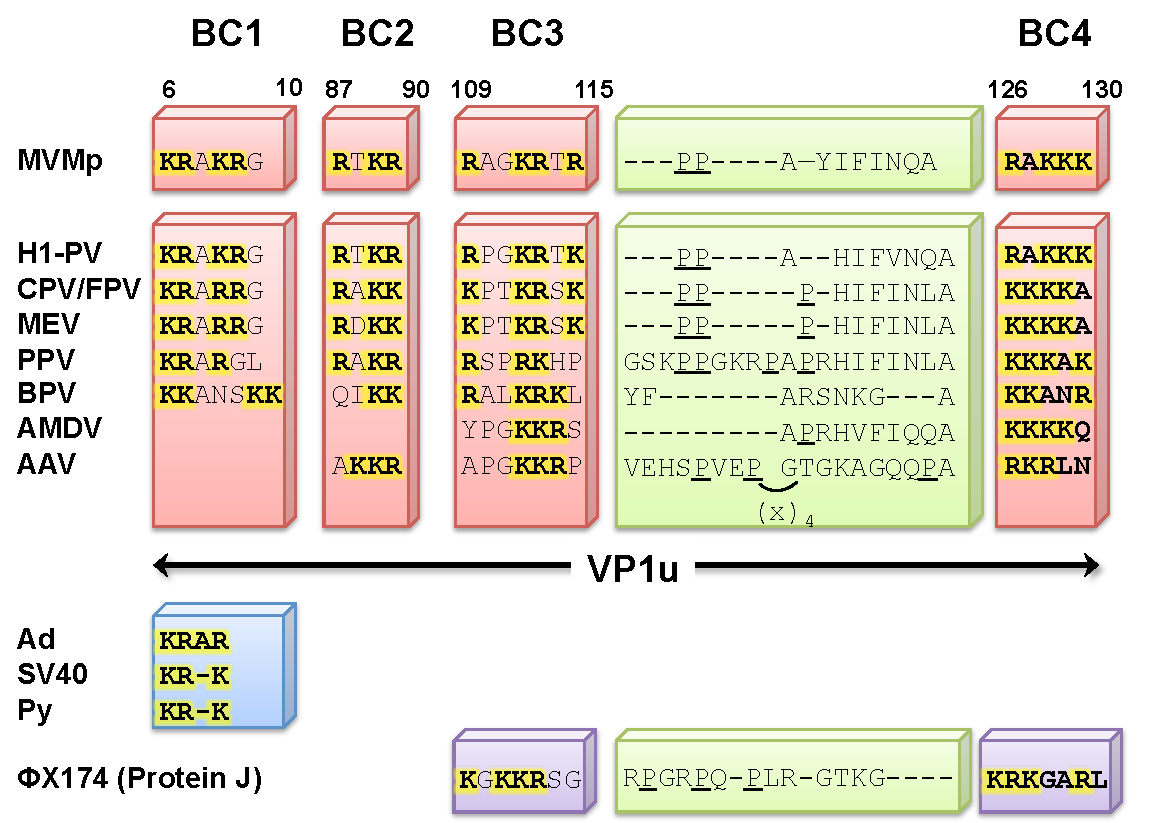
\includegraphics[scale=0.6]{NLS}
  \caption[Nuclear localisation signal (NLS)]
   {VP1 nuclear targeting sequences. The alignment of BCs (BC1 to BC4), which are conserved in the VP1u region among parvoviruses, is boxed in red. Amino acid residues are abbreviated using the single letter code. Sequence homology between BC1 and other karyophilic double-stranded DNA (dsDNA) viruses is shaded in blue on the left-hand side. Conservation of BC3 and BC4 with the protein J of the ssDNA bacteriophage $\phi$X174 is boxed in magenta on the right-hand side. Basic residues of the BC boxes are represented in bold face and possible homologous residues in the spacing region (boxed in green) between BC3 and BC4 are shadowed. Characteristic proline residues which are scattered along the space region are underlined. This illustration was adapted from \cite{pmid12072505, almendral}.}
\label{NLS}
\end{figure}


\subsection{The Nuclear Localization Motif (NLM)}
\label{NLM1}
Since both VP1 and VP2 singly expressed proteins efficiently target the nucleus of transfected cells \cite{pmid8416366, pmid12072505} each protein must carry its own nuclear transport sequence. The common C-terminal sequence of VP1 and VP2 lacks a conventional consensus NLS. However, VP2 contains one single region which is enriched in basic amino acids (528-KGKLTMRAKLR-538) near its C-terminus. Based on the crystal structure \cite{pmid9817841, pmid2006420}, analysis revealed that this sequence is structurally ordered as a $\beta$-sheet which forms the carboxy half of the $\beta$I strand (residues 520 to 538) of the eight-stranded antiparallel $\beta$-barrel (see Figure~\ref{NLM}, p.~\pageref{NLM}). Moreover, the $\beta$I-strand shows marked amphiphatic characteristics, exposing all the basic amino acids to the solvent in the interior surface of the capsid while the hydrophobic residues face toward the protein core. Mutational analysis revealed that the basic nature of the exposed face of $\beta$I, as well as the hydrophobic residues on the opposite face, conferred a nuclear localization capacity to the VP2 protein. Accordingly, this sequence in $\beta$I which only functions under a precise conformation, but not in a linear form, is referred to as the VP2 nuclear localization motif (NLM) \cite{pmid10729155}.        

\begin{figure}
\centering
  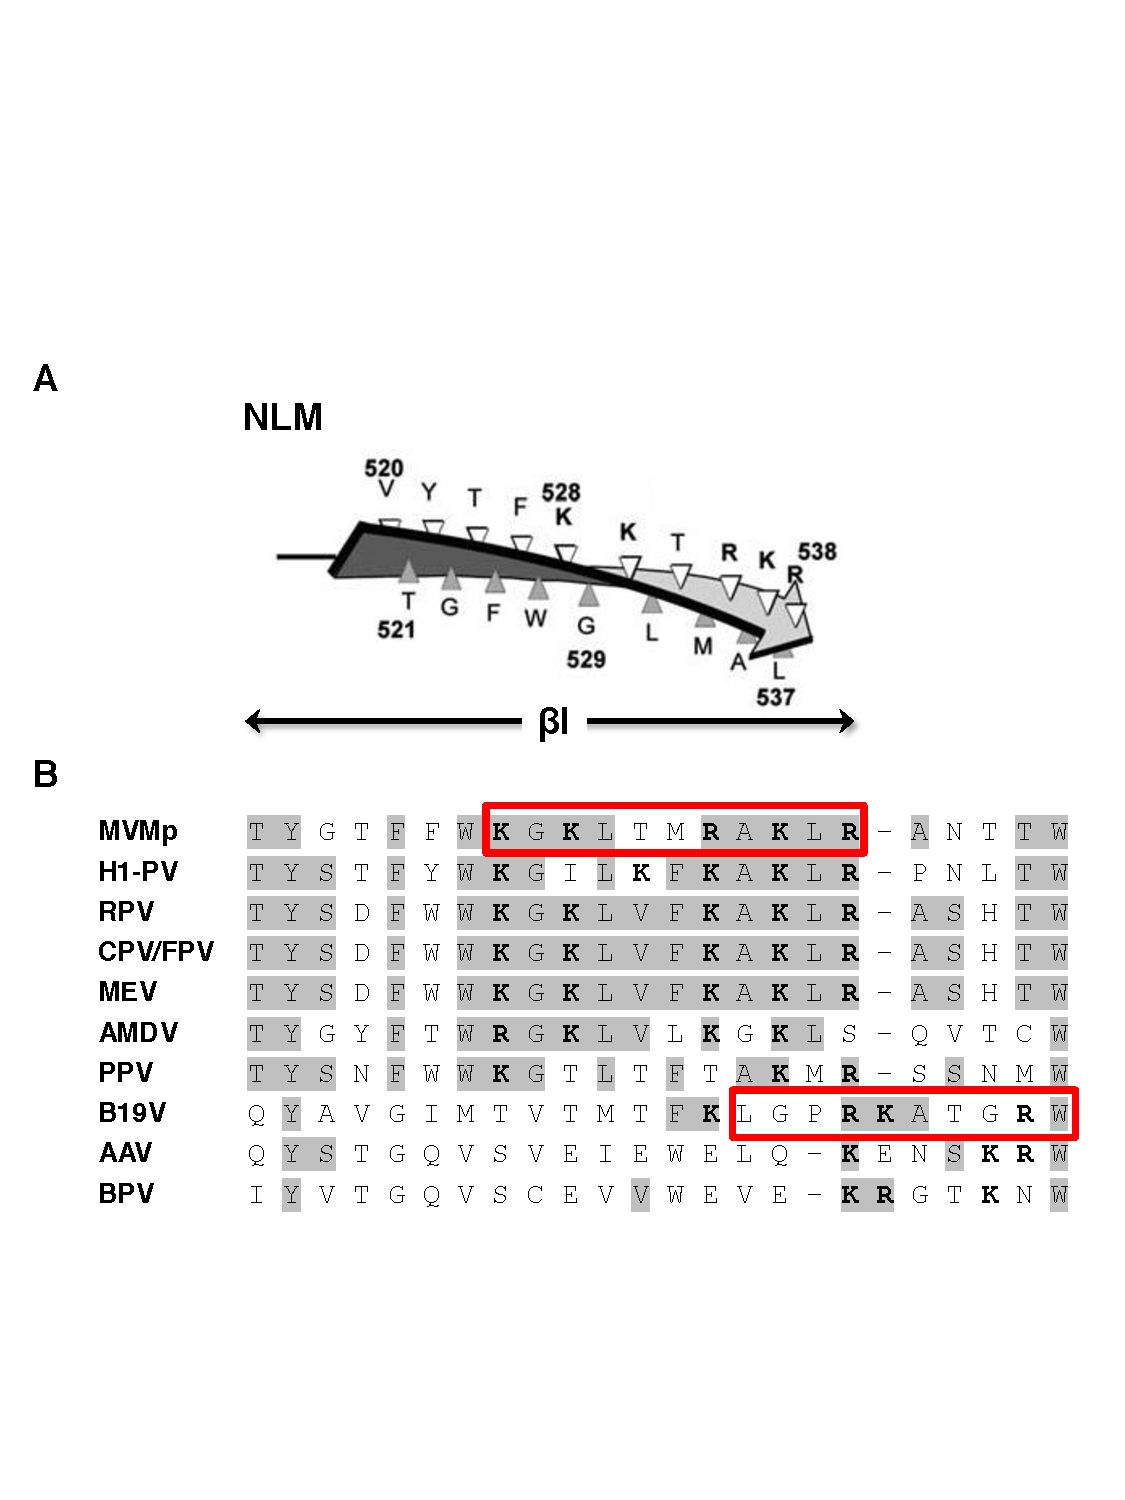
\includegraphics[scale=0.7]{NLM}[H!]
  \caption[Nuclear localisation motif (NLM)]
   {Nuclear localization motif (NLM). \textbf{(A)} Schematic representation of the VP2 NLM of MVM as disposed on the $\beta$-strand I of the antiparallel, eight-stranded $\beta$-barrel topology in the common C-terminal part of VP1 and VP2. Basic amino acids which are exposed to the solvent are represented in bold. \textbf{(B)} Alignment of the NLM that is conserved among parvoviruses. Homologous positions are shadowed and basic residues are in bold. Sequences with proven nuclear localization capacity are boxed in red. This illustration was adapted from \cite{pmid10729155, almendral}.} 
\label{NLM}
\end{figure}


\nomenclature{NLS}{Nuclear localization signal}
\nomenclature{NLM}{Nuclear localization motif}
\nomenclature{dsDNA}{Double-stranded DNA}
\nomenclature{ssDNA}{Single-stranded DNA}
\nomenclature{sPLA\textsubscript{2}}{Secretory PLA\textsubscript{2}}
\nomenclature{NPC}{Nuclear pore complex}
\nomenclature{BC}{Basic cluster}
\nomenclature{H1-PV}{Parvovirus H1}
\nomenclature{MW}{Molecular weight}
